\textit{Les probabilités demandées seront exprimées sous forme de fractions irréductibles.}

\medskip

\textbf{Partie A}

\medskip

On lance trois fois de suite une pièce de monnaie bien équilibrée. On note $X$ la variable aléatoire qui compte le nombre de fois, sur les trois lancers, où la pièce est retombée du côté « Face ».

\begin{enumerate}
	\item Préciser la nature et les paramètres de la loi de probabilité suivie par $X$.
	\item Recopier et compléter le tableau suivant donnant la loi de probabilité de $X$.
	
	\begin{Centrage}
		\begin{tblr}{width=0.975\linewidth,hlines,vlines,colspec={*{5}{X[m,c]}}}
			$k$ & 0 & 1 & 2 & 3 \\
			$P(X=k)$ &  &  &  &  \\
		\end{tblr}
	\end{Centrage}
\end{enumerate}

\textbf{Partie B}

\medskip

Voici les règles d'un jeu où le but est d'obtenir trois pièces du côté « Face » en un ou deux essais :

\begin{itemize}
	\item on lance trois pièces équilibrées :
	\begin{itemize}
		\item si les trois pièces sont tombées du côté « Face », la partie est gagnée ;
		\item sinon, les pièces tombées du côté « Face » sont conservées et on relance celles tombées du côté {«~Pile~»} ;
	\end{itemize}
	\item la partie est gagnée si on obtient trois pièces du côté « Face », sinon elle est perdue.
\end{itemize}

On considère les évènements suivants :

\begin{itemize}
	\item $G$ : « la partie est gagnée » ;
	
	et pour tout entier $k$ compris entre 0 et 3 , les évènements :
	\item $A_{k}$ : « $k$ pièces sont tombées du côté « Face » au premier lancer ».
\end{itemize}

\begin{enumerate}
	\item Démontrer que $P_{A_{1}}(G)=\frac{1}{4}$.
	\item Recopier et compléter l'arbre pondéré ci-dessous :
	
	\begin{Centrage}
		\begin{center}
			\begin{tikzpicture}
				\tikzstyle{fleche}=[->,>=latex,semithick]
				\tikzstyle{etiquette}=[fill=white,pos=0.6,inner sep=1.75pt,font=\small]
				\def\DistanceInterNiveaux{2.25}
				\def\DistanceInterFeuilles{0.85}
				\def\NiveauA{(0)*\DistanceInterNiveaux}
				\def\NiveauB{(1)*\DistanceInterNiveaux}
				\def\NiveauC{(2)*\DistanceInterNiveaux}
				\def\InterFeuilles{(-1)*\DistanceInterFeuilles}
				\coordinate (R) at ({\NiveauA},{(3)*\InterFeuilles}) ;
				\node[] (Ra) at ({\NiveauB},{(0.5)*\InterFeuilles}) {$A_0$};
				\node[] (Raa) at ({\NiveauC},{(0)*\InterFeuilles}) {$G$};
				\node[] (Rab) at ({\NiveauC},{(1)*\InterFeuilles}) {$\overline{G}$};
				\node[] (Rb) at ({\NiveauB},{(2.5)*\InterFeuilles}) {$A_1$};
				\node[] (Rba) at ({\NiveauC},{(2)*\InterFeuilles}) {$G$};
				\node[] (Rbb) at ({\NiveauC},{(3)*\InterFeuilles}) {$\overline{G}$};
				\node[] (Rc) at ({\NiveauB},{(4.5)*\InterFeuilles}) {$A_2$};
				\node[] (Rca) at ({\NiveauC},{(4)*\InterFeuilles}) {$G$};
				\node[] (Rcb) at ({\NiveauC},{(5)*\InterFeuilles}) {$\overline{G}$};
				\node[] (Rd) at ({\NiveauB},{(6)*\InterFeuilles}) {$A_3$};
				\node[] (Rda) at ({\NiveauC},{(6)*\InterFeuilles}) {$G$};
				% Arcs (MODIFIABLES : Styles)
				\draw[fleche] (R)--(Ra) node[etiquette] {$\tfrac18$};
				\draw[fleche] (Ra)--(Raa);
				\draw[fleche] (Ra)--(Rab);
				\draw[fleche] (R)--(Rb) node[etiquette] {$\tfrac38$};
				\draw[fleche] (Rb)--(Rba);
				\draw[fleche] (Rb)--(Rbb);
				\draw[fleche] (R)--(Rc) node[etiquette] {$\tfrac38$};
				\draw[fleche] (Rc)--(Rca);
				\draw[fleche] (Rc)--(Rcb);
				\draw[fleche] (R)--(Rd) node[etiquette] {$\tfrac18$};
				\draw[fleche] (Rd)--(Rda);
			\end{tikzpicture}
		\end{center}
		%:-+-+-+-+- Fin
	\end{Centrage}
	\item Démontrer que la probabilité $p$ de gagner à ce jeu est $p=\frac{27}{64}$
	\item La partie a été gagnée. Quelle est la probabilité qu'exactement une pièce soit tombée du côté « Face » à la première tentative?
	\item Combien de fois faut-il jouer à ce jeu pour que la probabilité de gagner au moins une partie dépasse $0,95$ ?
\end{enumerate}